\documentclass{acmsiggraph}

\usepackage{parskip}
\usepackage{graphicx}
\usepackage{footmisc}
\usepackage{amsmath}
\usepackage{url}
\onlineid{0}

\title{Cinematic Particle Systems with OpenCL}

\author{Tim Horton\thanks{e-mail: hortot2@rpi.edu}\\Rensselaer Polytechnic Institute}

\begin{document}

\maketitle

\begin{figure}
    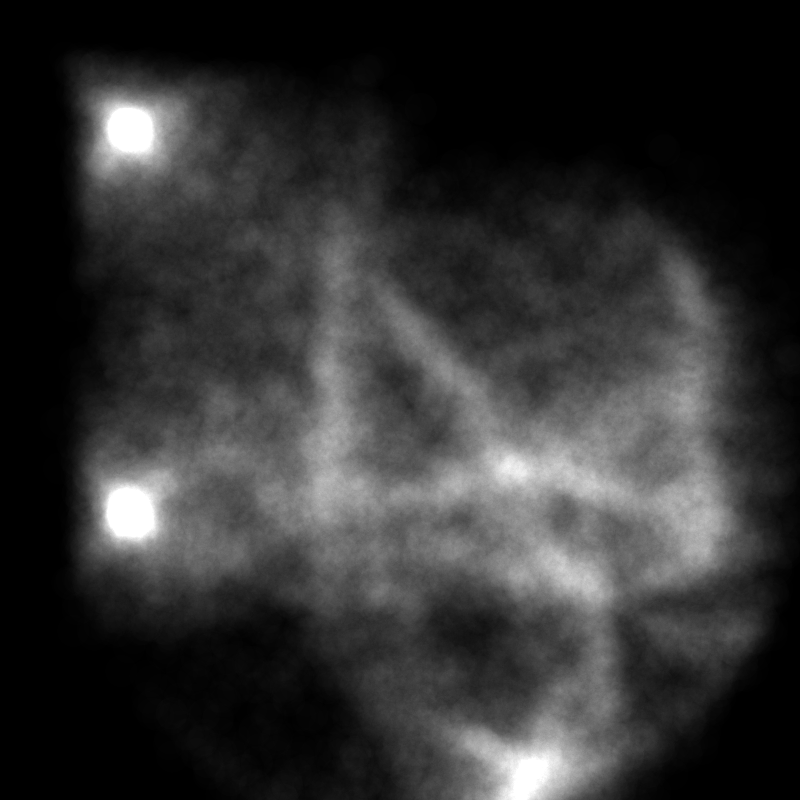
\includegraphics[width=84.5mm]{gravity.png}
    \caption{A gravity simulation with two emitters and three supermassive particles (approx. 45,000 particles)}
\end{figure}

\section*{Abstract}

High-particle-count simulations are becoming increasingly crucial in many different aspects of our world today: both in entertainment --- within video games, movies, and the like --- and in scientific fields, where particle systems are capable of simulating and visualizing many interesting phenomena.

This paper will explore the possibility of parallelizing the simulation of these large particle systems and offloading them to very-parallel\footnote{As opposed to {\it massively-}parallel, like the CCNI's Blue Gene/L, or the {\it slightly}-parallel CPU in most modern computers} hardware which is usually only used for {\it rendering}: the video card.

We will also touch briefly on ways to design a system for describing particle systems in a generalized way, though the majority of the work that is currently in a functional state centers around simulation and rendering.

\section{Introduction}

Simulation of large particle systems requires a large amount of computation --- each particle must be inspected and updated. For certain types of particle systems --- n-body gravity, for example --- each particle is affected by its neighbors, increasing the required calculation time drastically.

This is what we aim to address with this paper. While it's unlikely that we can contribute any improved simulation algorithms, we can instead work to parallelize these algorithms and implement them with OpenCL, which will allow them to run on the GPU contained within modern graphics cards. This paper will demonstrate both the parallelization of the application of forces on large numbers of particles and the significant performance gained by doing so.

We will also explore a simple parallelized particle renderer, as well as the potential for the integration of our simulator into the popular open-source 3D package, Blender.

\section{Prior Art}

\section{Implementation}

The code for this paper is available under the 2-clause BSD license at:

\url{http://github.com/hortont424/particles}

It consists of about 3000 lines of C and Objective C, which encompass the curve editor and other design tools, an abstraction layer on top of OpenCL, and all of the code to drive simulation, preview, and rendering. In addition, there are about 350 {\bf [UPDATE THIS]} lines of OpenCL Kernel Language, which includes the code to apply each of the forces as well as the renderer.

\subsection{Design}

\subsection{Simulation}

\subsubsection{Physics}

\subsection{Preview}

\subsection{Rendering}

\section{Performance \& Results}

\subsection{Hardware}

\subsection{Benchmarks}

\subsection{Video}

\section{Applications}

\section{Future Work}

\subsection{Spatial Hashing}

\subsection{Design Tools}

\subsection{Extended Properties}

\subsection{Rendering Improvements}

\subsection{Blender Integration}

\section{Conclusion}

\bibliographystyle{acmsiggraph}
\nocite{*}
\bibliography{report}

\end{document}